\documentclass{beamer}

\usepackage[utf8]{inputenc}

\usepackage{graphicx} %For images
\graphicspath{ {./images/} }


\setbeamertemplate{navigation symbols}{}%remove navigation symbols

\title[Predictive Model] %optional
{Predictive Model for Traffic Control in Underground Mines}

\author{Claes Andersson \\\small Supervisors: \\ Olov Schelén \and Johan Kristiansson}

\institute[LTU] % (optional)
{Luleå University of Technology \and Mobilaris MCE}

\date{June 3, 2019}

\logo{
\includegraphics[height=0.8cm]{mobilaris_logo.png}}

\begin{document}
	\frame{\titlepage}

	\begin{frame}
		\frametitle{Mine Conditions}
		\begin{columns}
			\column{0.4\textwidth}
			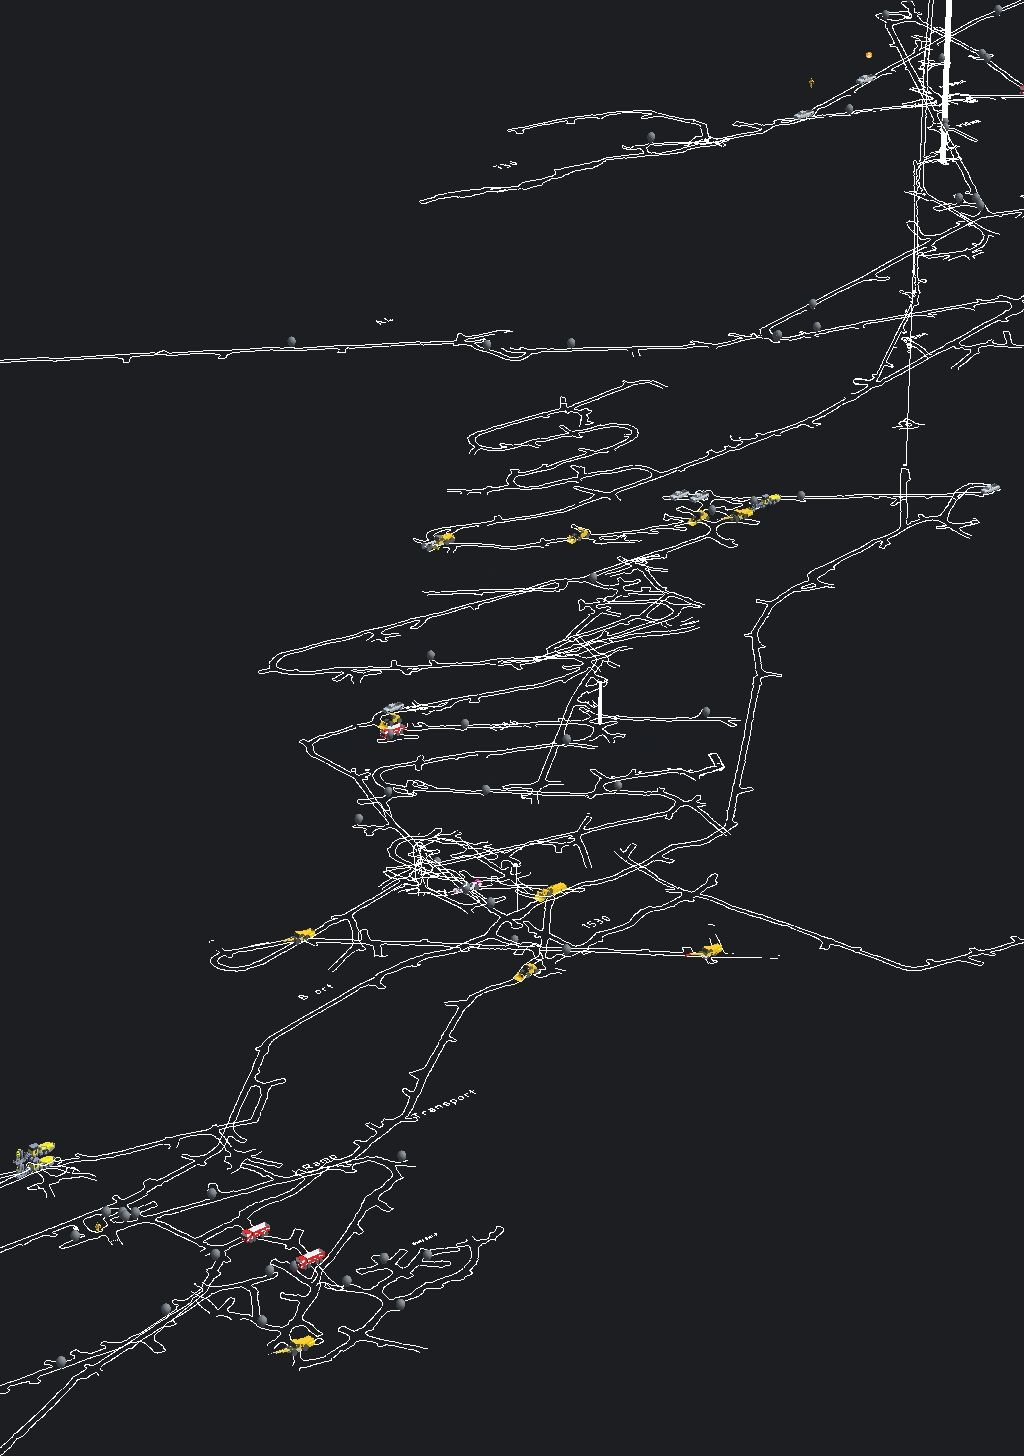
\includegraphics[height=0.8\textheight]{onboard.jpg}
			\column{0.5\textwidth}
				\begin{itemize}
					\item Lots of people and vehicles
					\item Deep below ground
					\item No radio penetration
					\item WiFi
				\end{itemize}
		\end{columns}
	\end{frame}

	{
	\setbeamercolor{background canvas}{bg=black}
	\setbeamertemplate{logo}{}
	\begin{frame}
		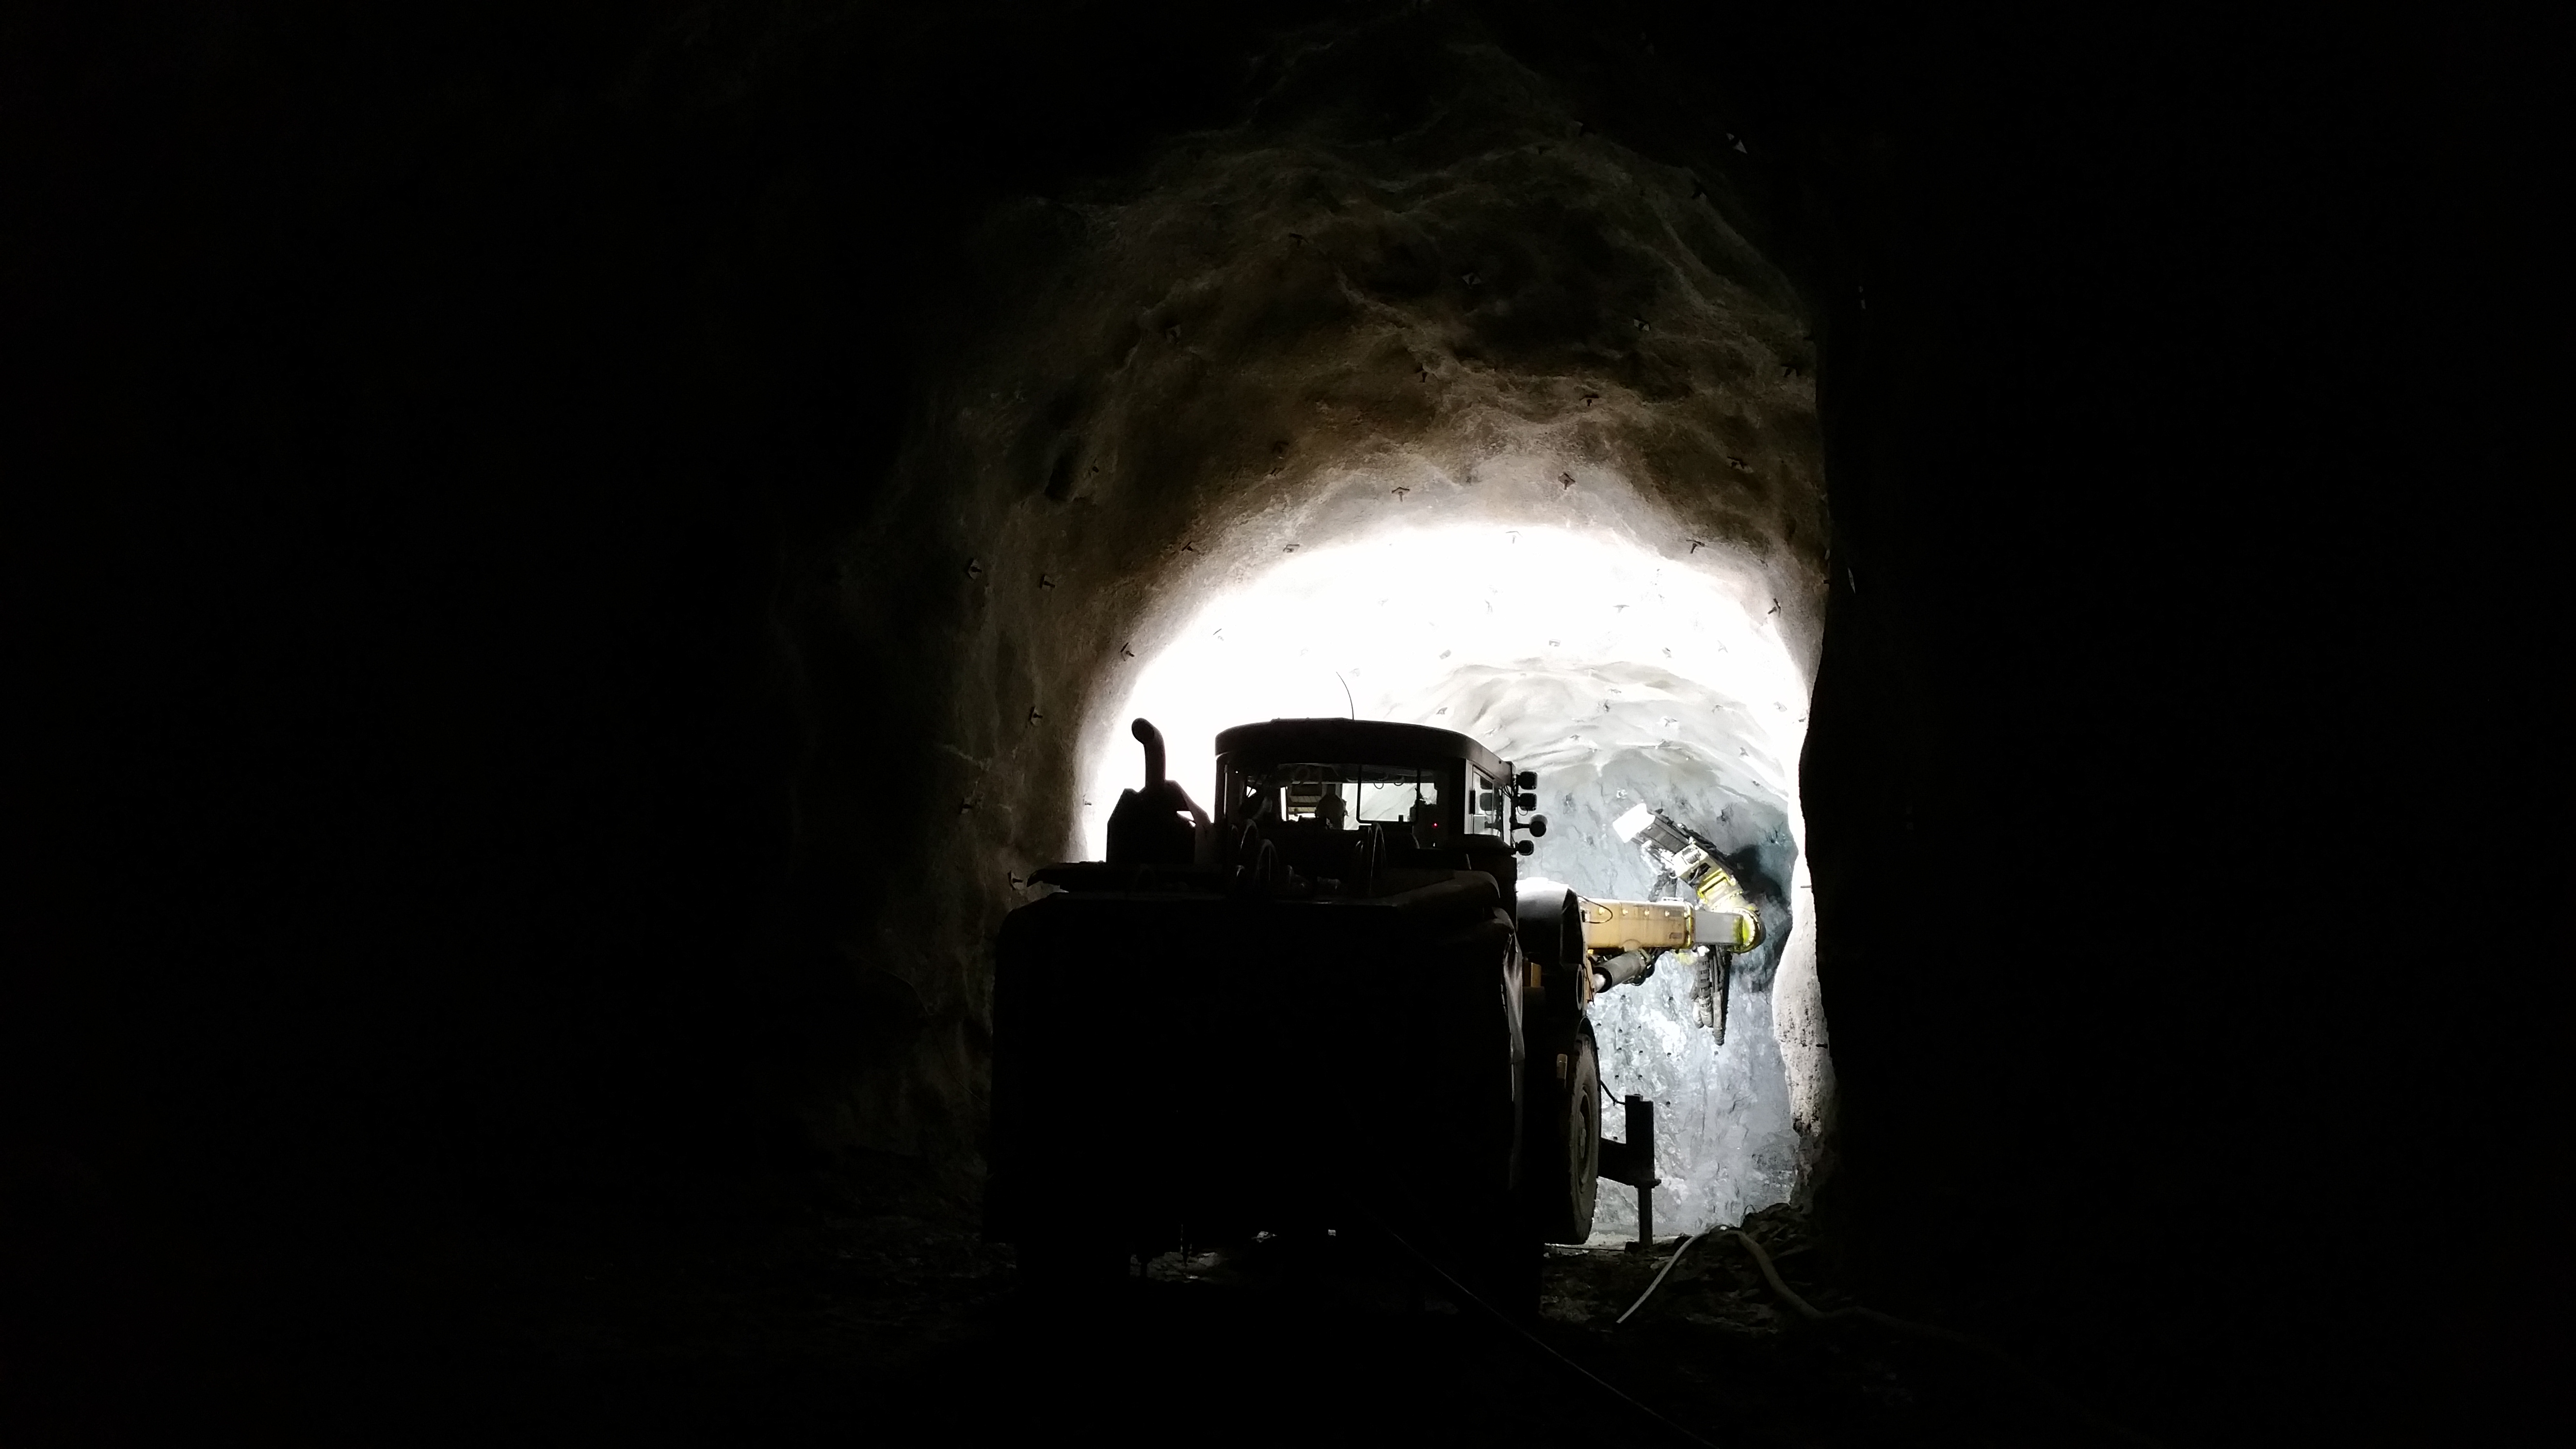
\includegraphics[width=\textwidth,height=\textheight,keepaspectratio]{diggingTunnel.jpg}
	\end{frame}
	}
%	\setbeamercolor{background canvas}{bg=white}
	\begin{frame}
		\frametitle{Narrow Roads}
		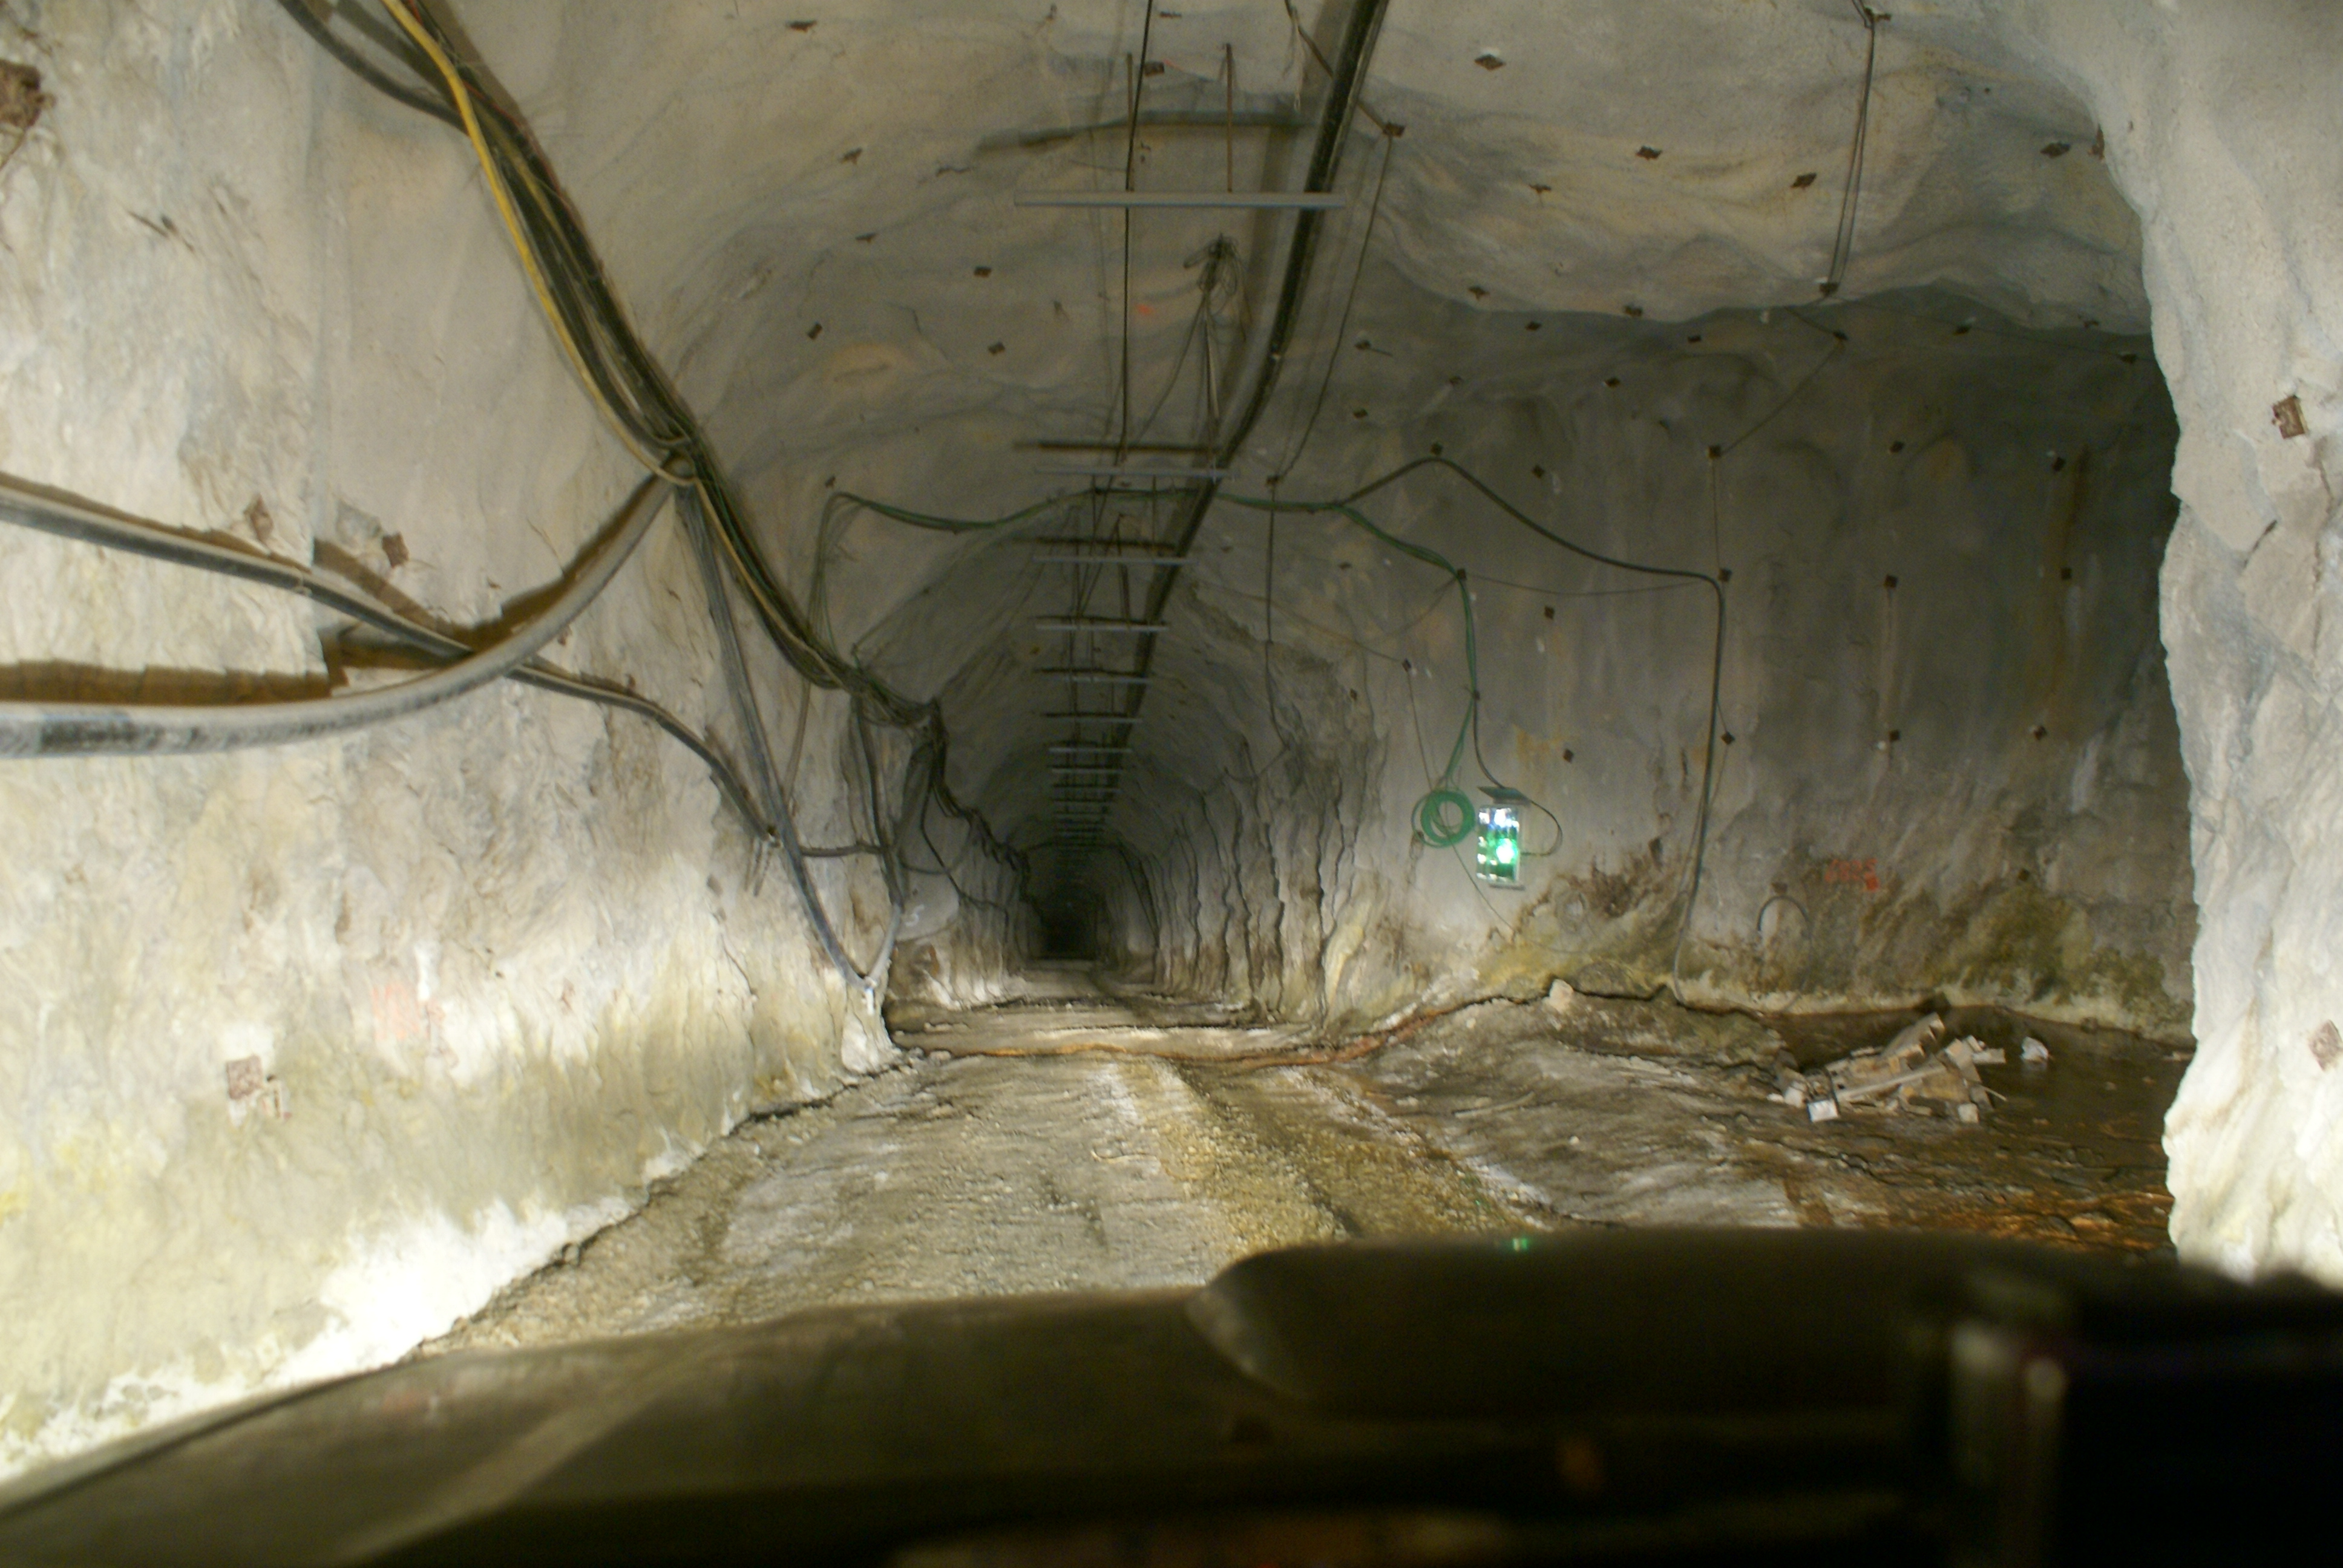
\includegraphics[width=\textwidth,height=\textheight,keepaspectratio]{mineRoad.jpg}
	\end{frame}

	\begin{frame}
		\frametitle{Problem Breakdown}
		\begin{itemize}
			\item Identify oncoming vehicles
			\item Identify nearby meeting slots or places to give way
			\item Predict difference in arrival time to a meeting slot
			\item Manage inaccurate positioning
			\item Manage loss of connection and old data
		\end{itemize}
	\end{frame}

	\begin{frame}
		\frametitle{Avaliable Resources}
		\begin{itemize}
			\item A graph representation of the map.
			\item Positioning for every vehicle in the mine.
			\item History of previous travel in form of logs.
		\end{itemize}
	\end{frame}

	\begin{frame}
		\frametitle{Log Structure}
		\begin{center}
			\begin{tabular}{|l|l|l|l|l| lll}
				\hline
				time & speed & x & y & z &.&.&.\\
				\hline
				553 & 22 & 1340 & 543 & -430 &.&.&. \\
				554 & 20 & 1338 & 547 & -431 &.&.&.\\
				555 & 18 & 1336 & 550 & -431 &.&.&.\\
				556 & 20 & 1335 & 556 & -432 &.&.&.\\
				557 & 21 & 1335 & 556 & -432 &.&.&.\\
				558 & 23 & 1333 & 560 & -434 &.&.&.\\
				559 & 24 & 1333 & 563 & -435 &.&.&.\\
				560 & 24 & 1330 & 563 & -436 &.&.&.\\
				561 & 26 & 1330 & 560 & -436 &.&.&.\\
				562 & 25 & 1328 & 557 & -437 &.&.&.\\
				563 & 25 & 1330 & 555 & -438 &.&.&.\\
				.&.&.&.&.&&&\\
				.&.&.&.&.&&&\\
				.&.&.&.&.&&&\\

			\end{tabular}

		\end{center}
	\end{frame}

	\begin{frame}
%		\frametitle{Speed: Random Variable}
		\frametitle{Gaussian Assumption of Speed over Edge}
		\begin{center}
%			{\large\bfseries Gaussian assumption} \\
			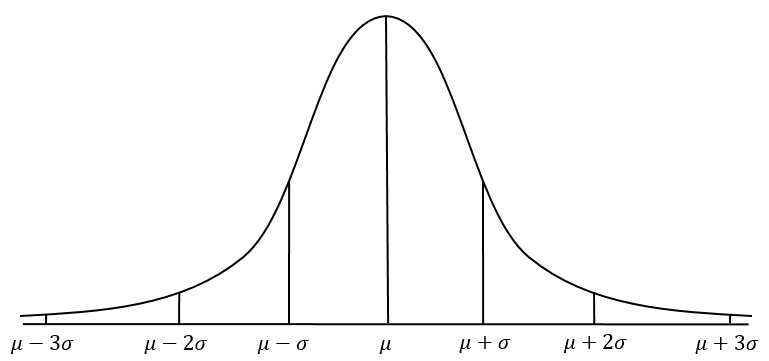
\includegraphics[width=0.8\textwidth]{normalDist2.png}
			\\$Speed \sim N(\mu, \sigma)$
			\pause
			\\Dependent or independent?
			\pause
			\\[0.5cm]Time over edge $= \frac{Distance}{Speed}$
		\end{center}
	\end{frame}

	\begin{frame}
		\frametitle{Linarising Distance over Speed}
		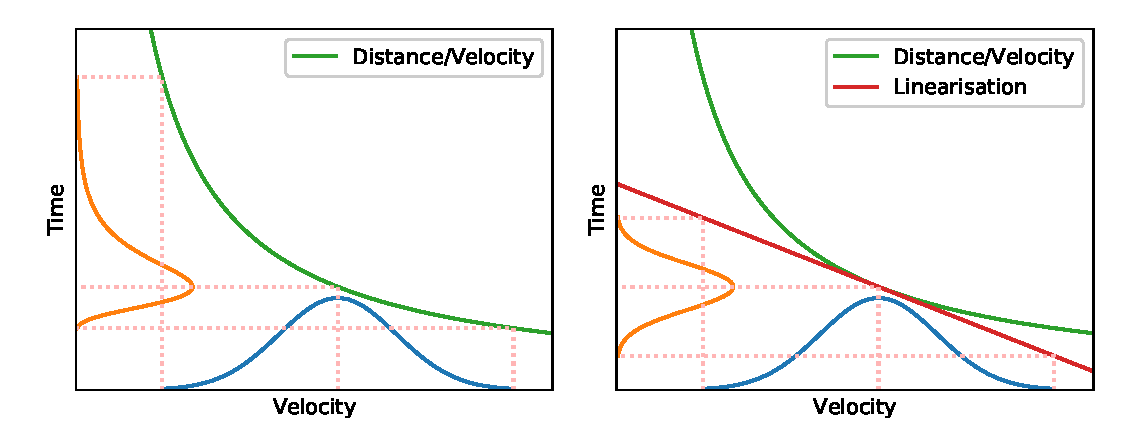
\includegraphics[width=\textwidth]{linearisation.eps}
	\end{frame}

	\begin{frame}
		\frametitle{Adding time of Path}
		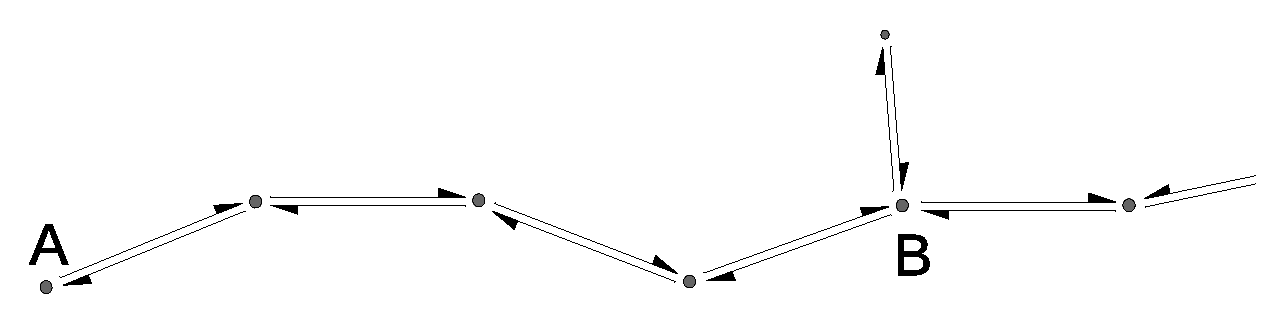
\includegraphics[width=\textwidth]{simpleDCEL.eps}
		\vspace{0.3cm}
		\begin{equation*}
			time = \frac{Distance_1}{Speed_1}+\frac{Distance_2}{Speed_2}+ ... +\frac{Distance_n}{Speed_n}
		\end{equation*}
	\end{frame}

	\begin{frame}
		\frametitle{Result Layout}
		{ Results:}
		\begin{itemize}
			\item Edge speed distributions\\\hspace{0.3cm}How well do they reflect reality?
			\item Linearisation and dependence\\\hspace{0.3cm}How much do they distort the results?
			\item Predicting time difference to a point\\\hspace{0.3cm}How well does it work?
		\end{itemize}
	\end{frame}

	\begin{frame}
		\frametitle{Edge Speed Distribution Results}
		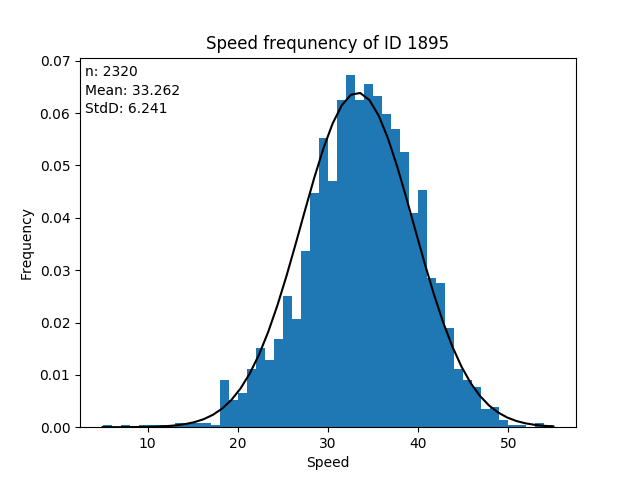
\includegraphics[width=\textwidth,height=\textheight,keepaspectratio]{logResGood.png}
	\end{frame}
	\begin{frame}
		\frametitle{Edge Speed Distribution Results}
		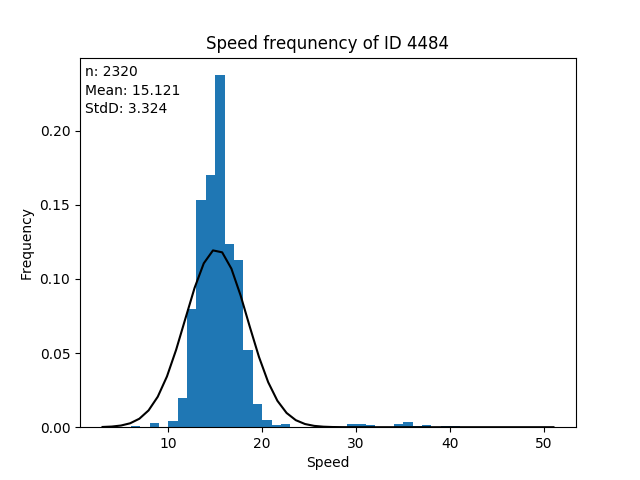
\includegraphics[width=\textwidth,height=\textheight,keepaspectratio]{logResEh1.png}
	\end{frame}
	\begin{frame}
		\frametitle{Edge Speed Distribution Results}
		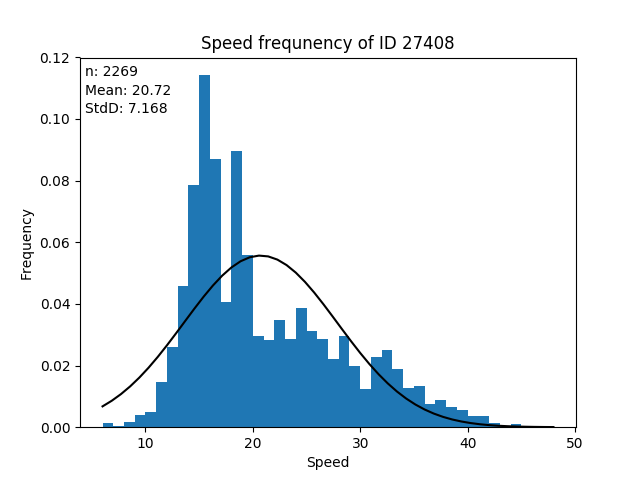
\includegraphics[width=\textwidth,height=\textheight,keepaspectratio]{logResEh2.png}
	\end{frame}
	\begin{frame}
		\frametitle{Edge Speed Distribution Results}
		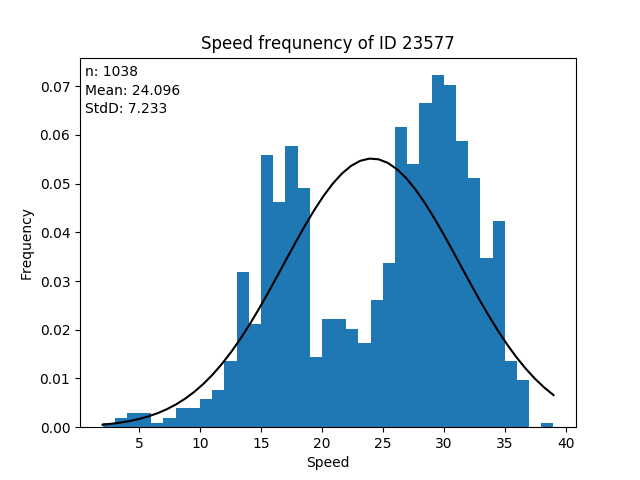
\includegraphics[width=\textwidth,height=\textheight,keepaspectratio]{logResBad.png}
	\end{frame}

	\begin{frame}
		\frametitle{Comparing against logs}
		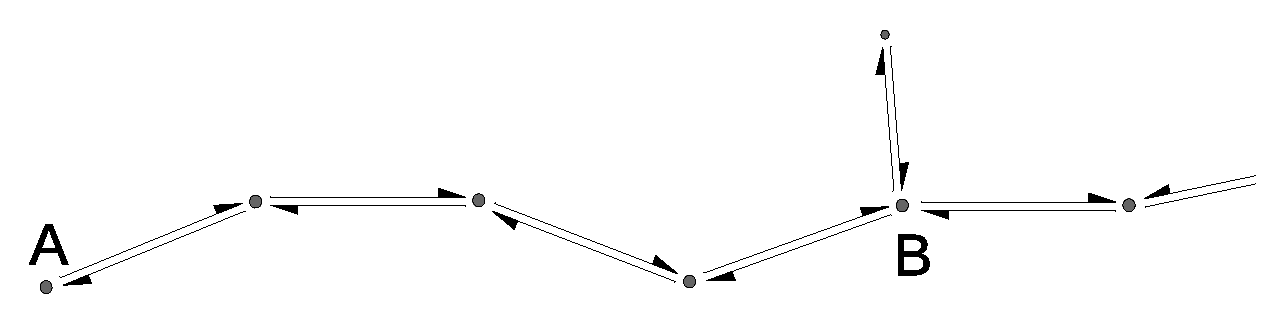
\includegraphics[width=\textwidth]{simpleDCEL.eps}
		\\\vspace{0.5cm}
		\begin{center}
			Set of logs from A to B vs Prediction
			\begin{itemize}
				\centering
				\item[]<2-> Log Time
				\item[]<3-> Log Speed
				\item[]<4-> Theory
			\end{itemize}
		\end{center}
	\end{frame}

	\begin{frame}
		\frametitle{Linearisation and Dependence, Short}
		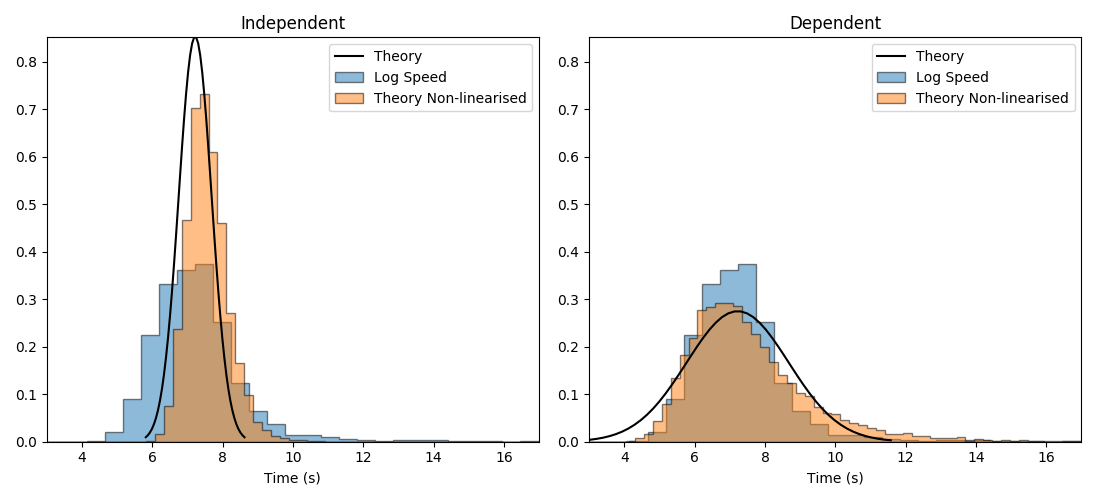
\includegraphics[width=\textwidth,height=\textheight,keepaspectratio]{non-lin10-10A.png}
		Path 10 edges long
	\end{frame}
	\begin{frame}
		\frametitle{Linearisation and Dependence, Short}
		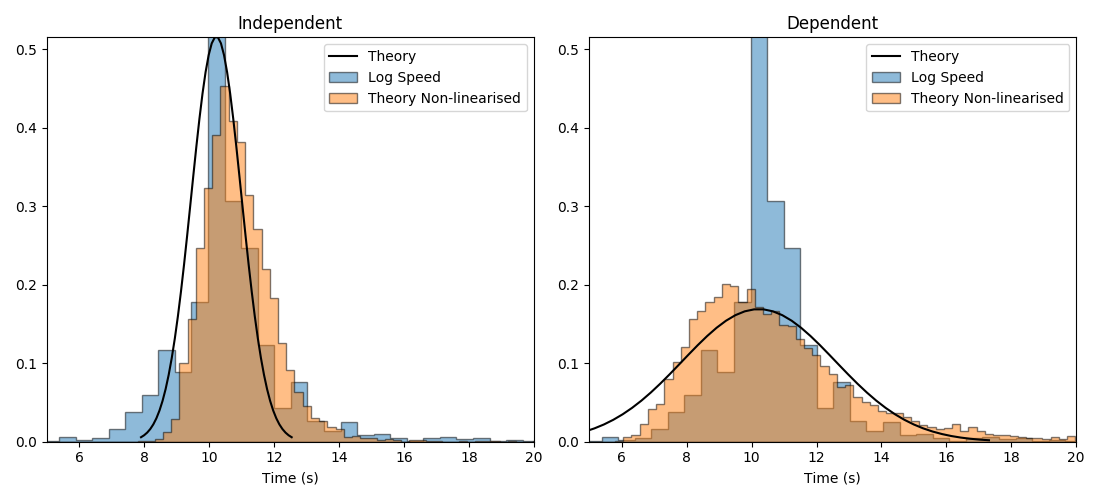
\includegraphics[width=\textwidth,height=\textheight,keepaspectratio]{non-lin10-10B.png}
		Path 10 edges long
	\end{frame}
	\begin{frame}
		\frametitle{Linearisation and Dependence, Short}
		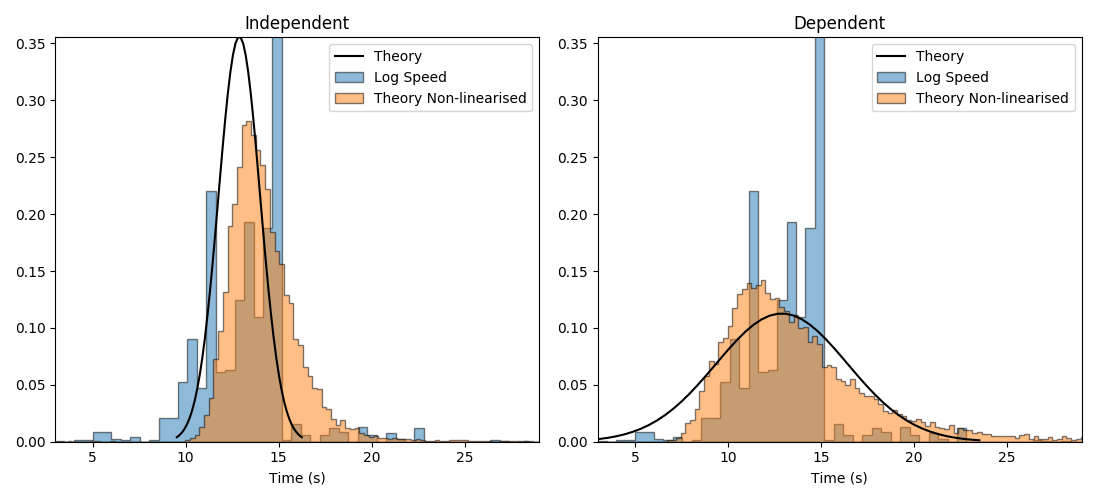
\includegraphics[width=\textwidth,height=\textheight,keepaspectratio]{non-lin8-10A.png}
		Path 10 edges long
	\end{frame}

	\begin{frame}
		\frametitle{Linearisation and Dependence, Long}
		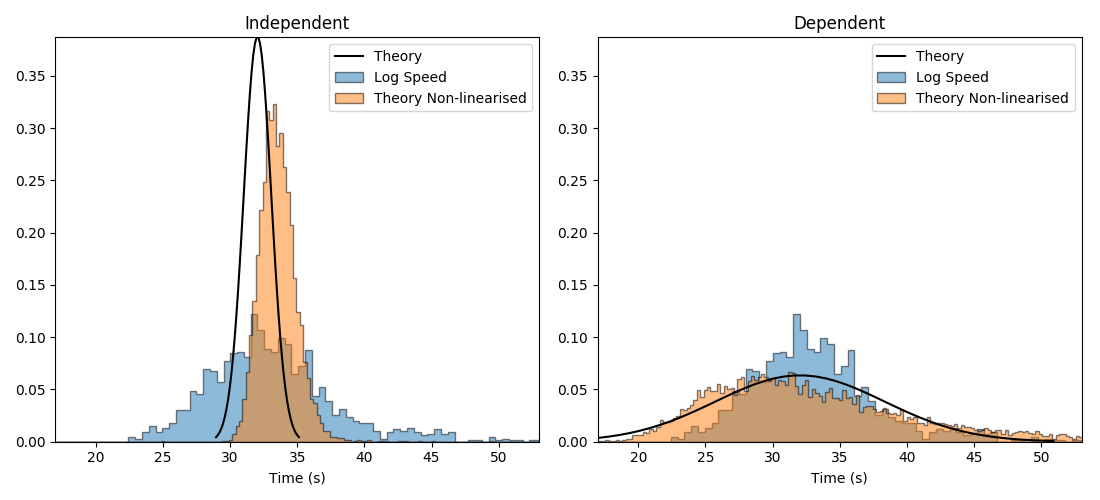
\includegraphics[width=\textwidth,height=\textheight,keepaspectratio]{non-lin10-40B.png}
		Same path that had good independent fit, now 40 edges long
	\end{frame}
	\begin{frame}
		\frametitle{Linearisation and Dependence, Long}
		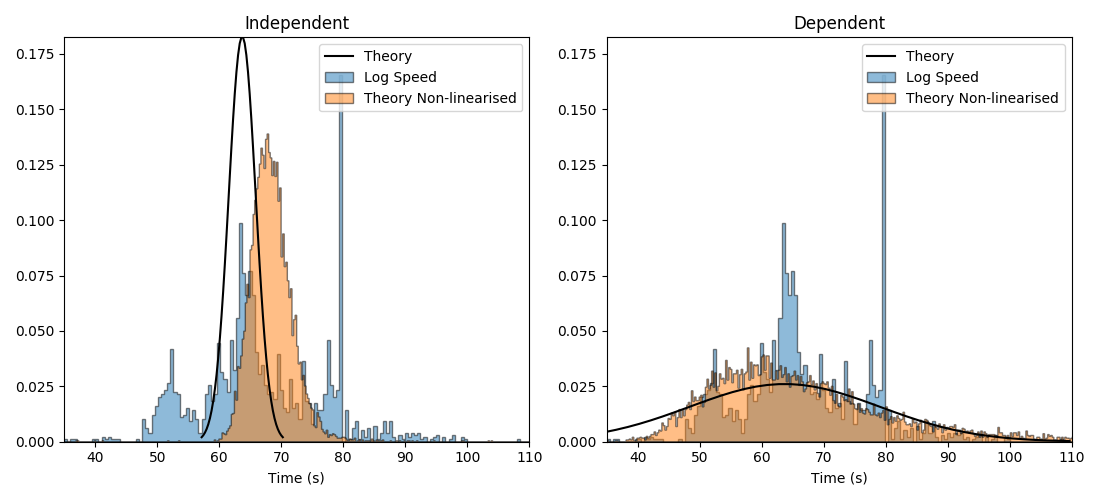
\includegraphics[width=\textwidth,height=\textheight,keepaspectratio]{non-lin8-50A.png}
		Same path that didn't have a good gaussian fit, now 50 edges long
	\end{frame}
	\begin{frame}
		\frametitle{Linearisation and Dependence, Long}
		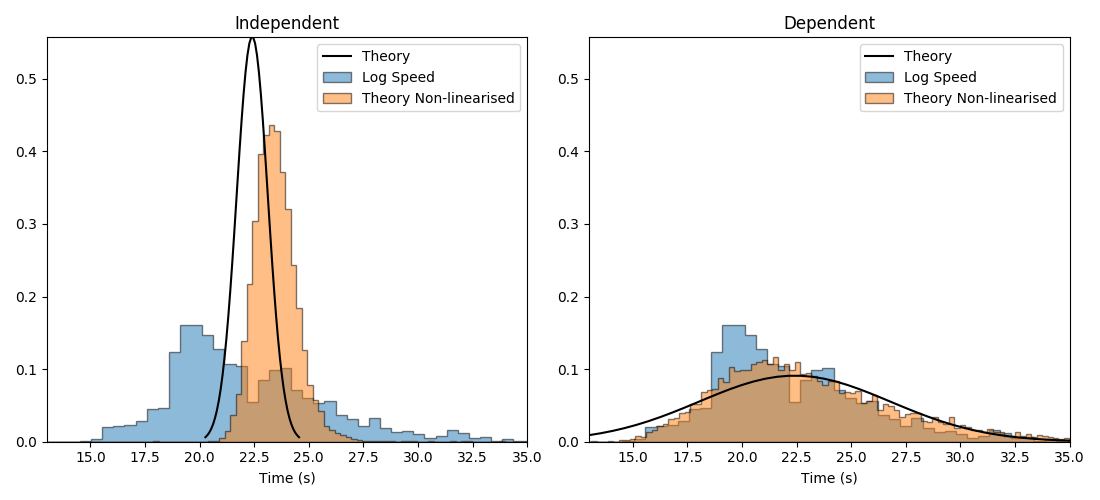
\includegraphics[width=\textwidth,height=\textheight,keepaspectratio]{non-lin12-40A.png}
		40 edges long path. Slanted Log Speed.
	\end{frame}

	\begin{frame}
		\frametitle{Time Differnece of Two Paths}
		\hspace{1.6cm}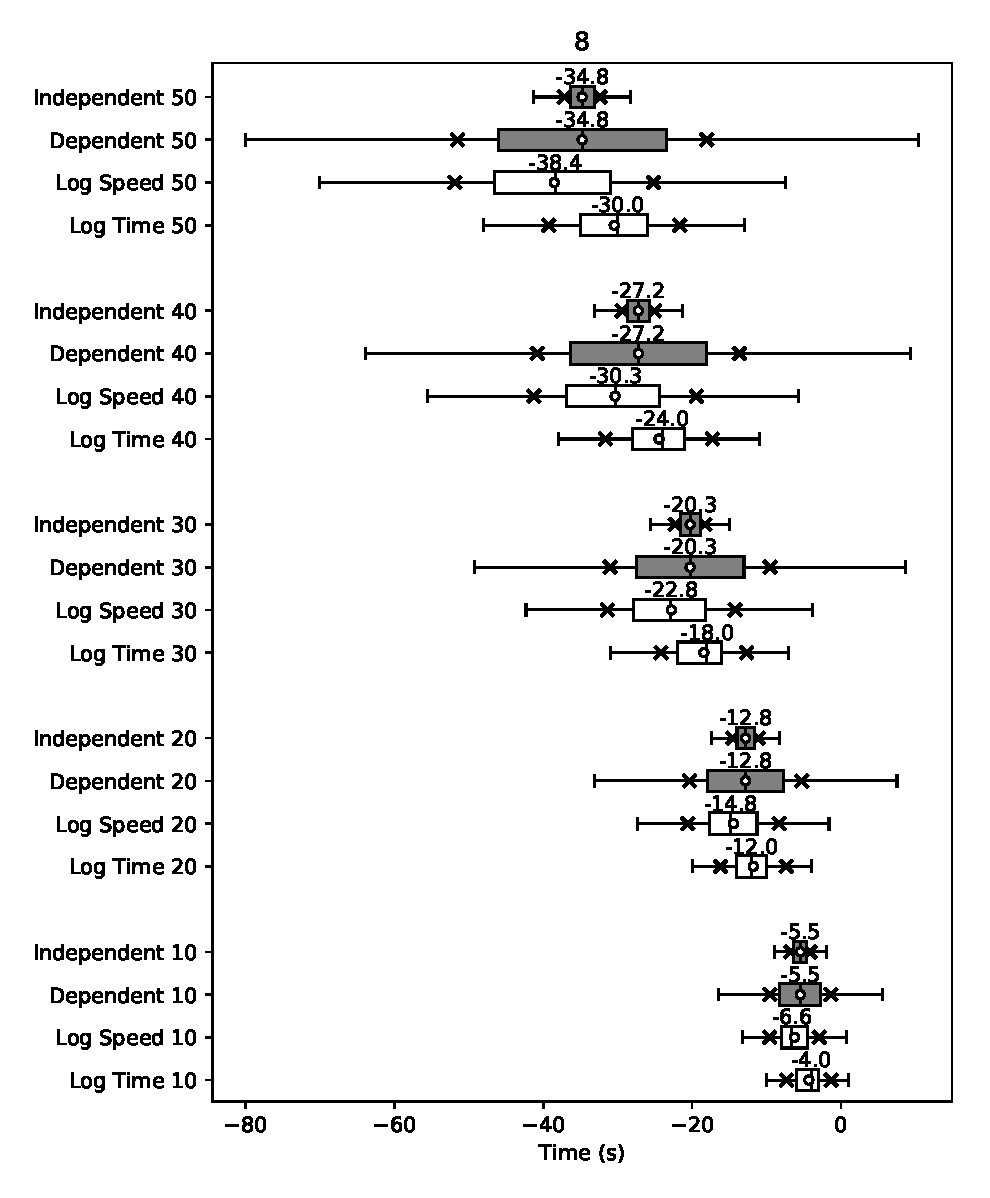
\includegraphics[height=0.8\textheight]{8.eps}
	\end{frame}

	\begin{frame}
		\frametitle{Conclusion}
		\LARGE
		\begin{itemize}
			\item The good
			\item The bad
			\item The ugly
		\end{itemize}
	\end{frame}

	\section{Appendix}

	\begin{frame}
		\frametitle{Appendix - Data}
			\begin{tabular}{ll}
				Number of nodes: & 16433\\
				Number of edges: & 32956\\
				Files processed: & 836 \\
				Total points of data: & 8627650\\
				Biggest single dataset: & 3341\\
			\end{tabular}
	\end{frame}

	\begin{frame}
		\frametitle{Appendix - Code}
		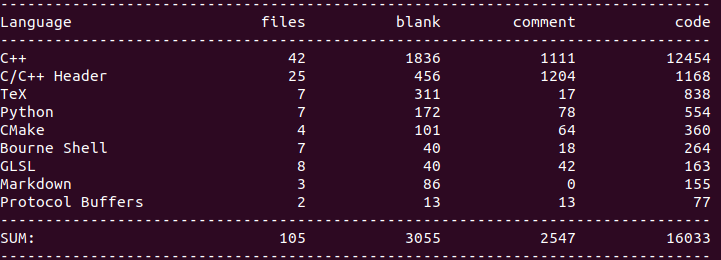
\includegraphics[width=\textwidth,height=\textheight,keepaspectratio]{cloc.png}
	\end{frame}
	\begin{frame}
		\frametitle{Appendix - More Time Differences}
		\hspace{1.6cm}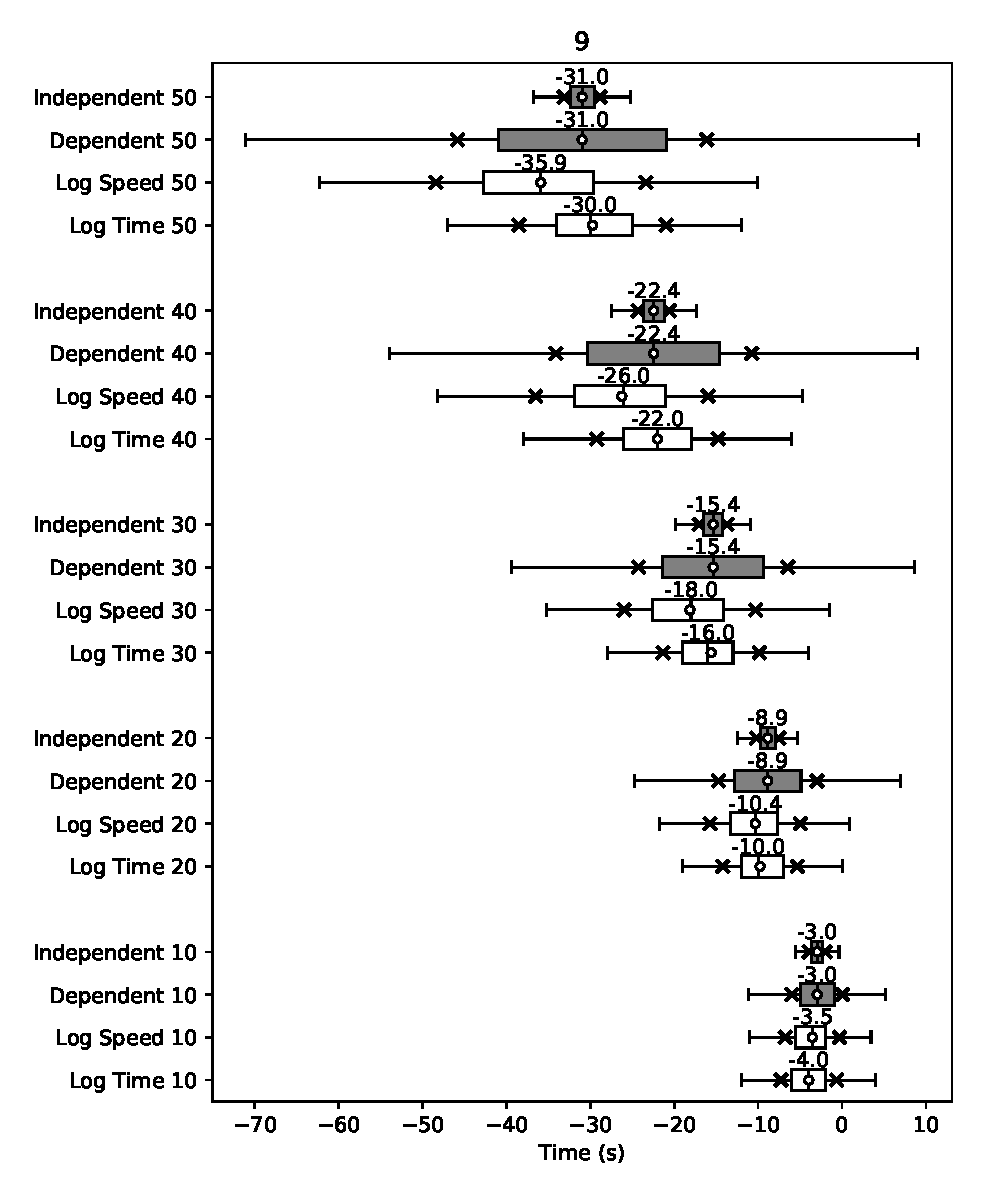
\includegraphics[height=0.8\textheight]{9.eps}
	\end{frame}
	\begin{frame}
		\frametitle{Appendix -  More Time Differences}
		\hspace{1.6cm}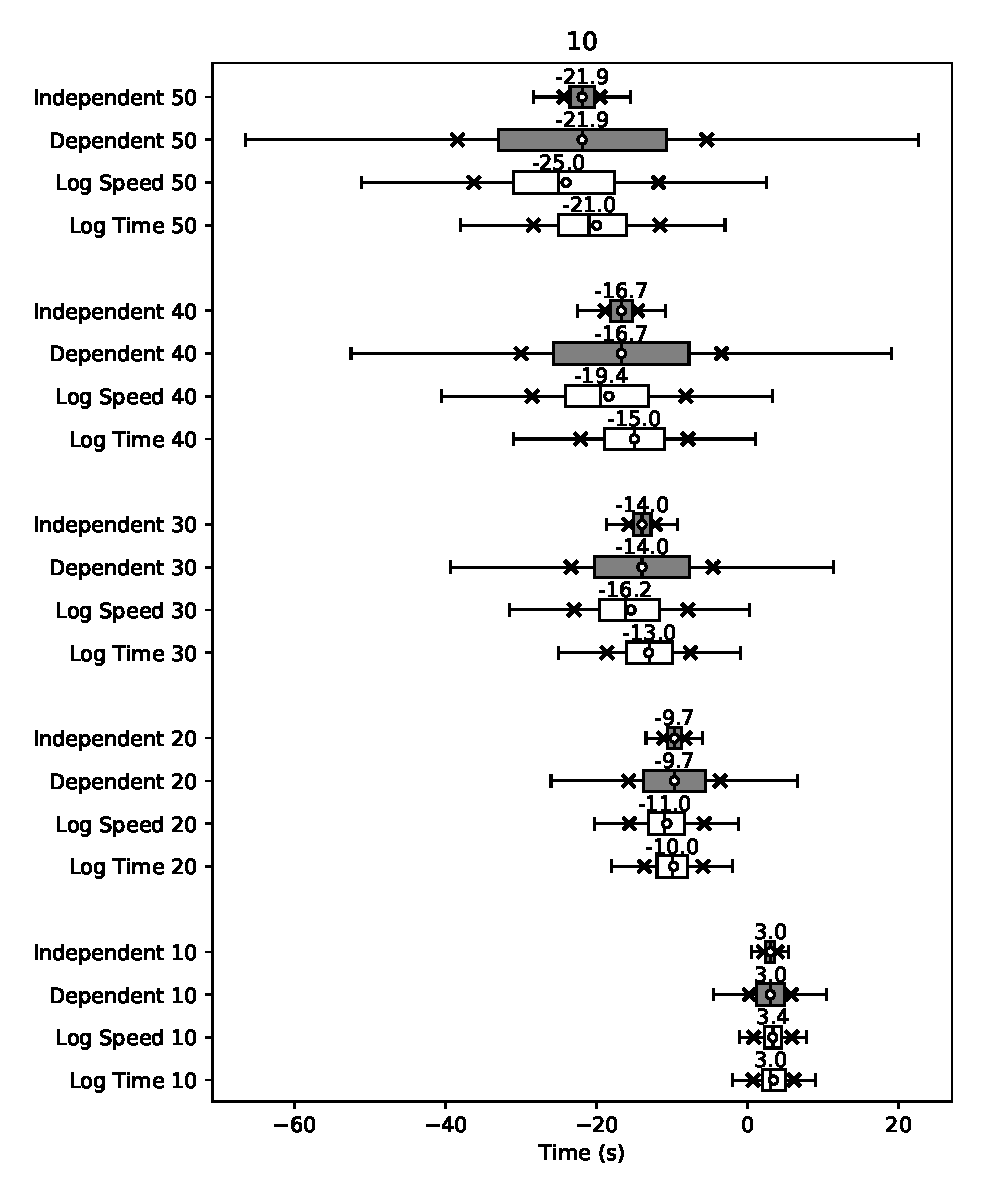
\includegraphics[height=0.8\textheight]{10.eps}
	\end{frame}
	\begin{frame}
		\frametitle{Appendix -  Time Difference Distribution}
		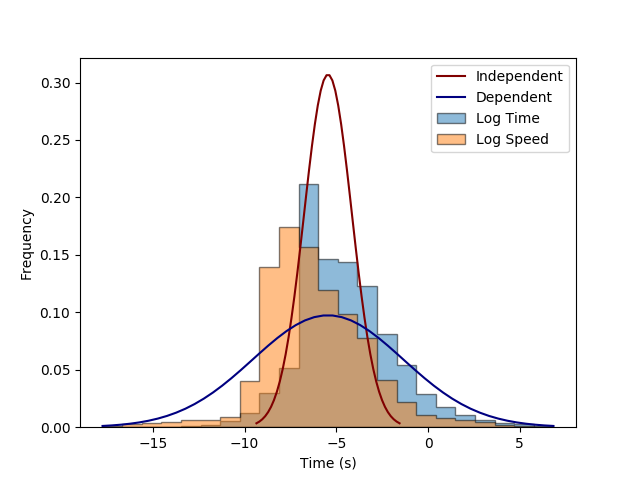
\includegraphics[width=\textwidth,height=\textheight,keepaspectratio]{DiffDist-8-10.png}
		10 Edges
	\end{frame}
	\begin{frame}
		\frametitle{Appendix -  Time Difference Distribution}
		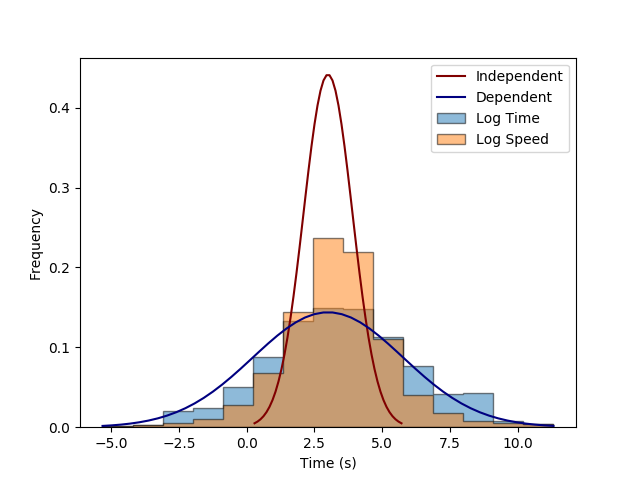
\includegraphics[width=\textwidth,height=\textheight,keepaspectratio]{DiffDist-10-10.png}
		10 Edges
	\end{frame}
	\begin{frame}
		\frametitle{Appendix -  Time Difference Distribution}
		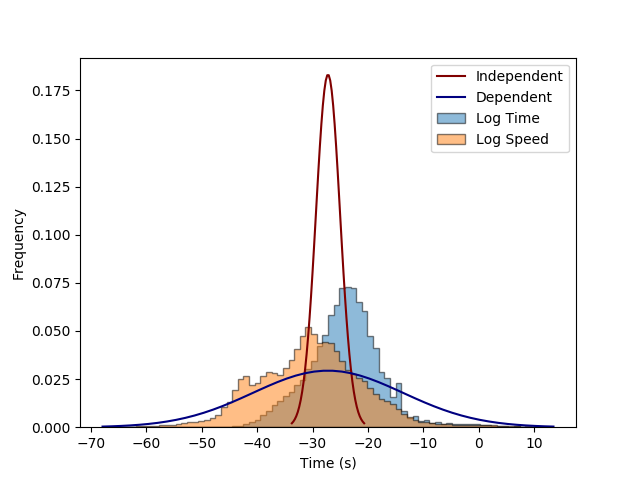
\includegraphics[width=\textwidth,height=\textheight,keepaspectratio]{DiffDist-8-40.png}
		40 Edges
	\end{frame}
	\begin{frame}
		\frametitle{Appendix -  Time Difference Distribution}
		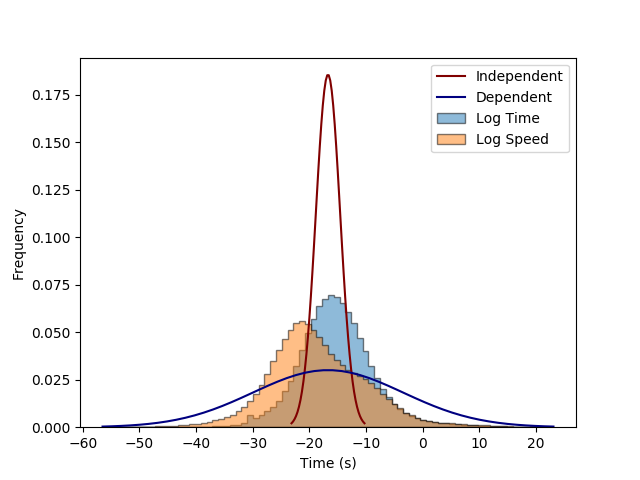
\includegraphics[width=\textwidth,height=\textheight,keepaspectratio]{DiffDist-10-50.png}
		50 Edges
	\end{frame}
	\begin{frame}
		\frametitle{Appendix - Old Data Time Differences}
		\hspace{1.6cm}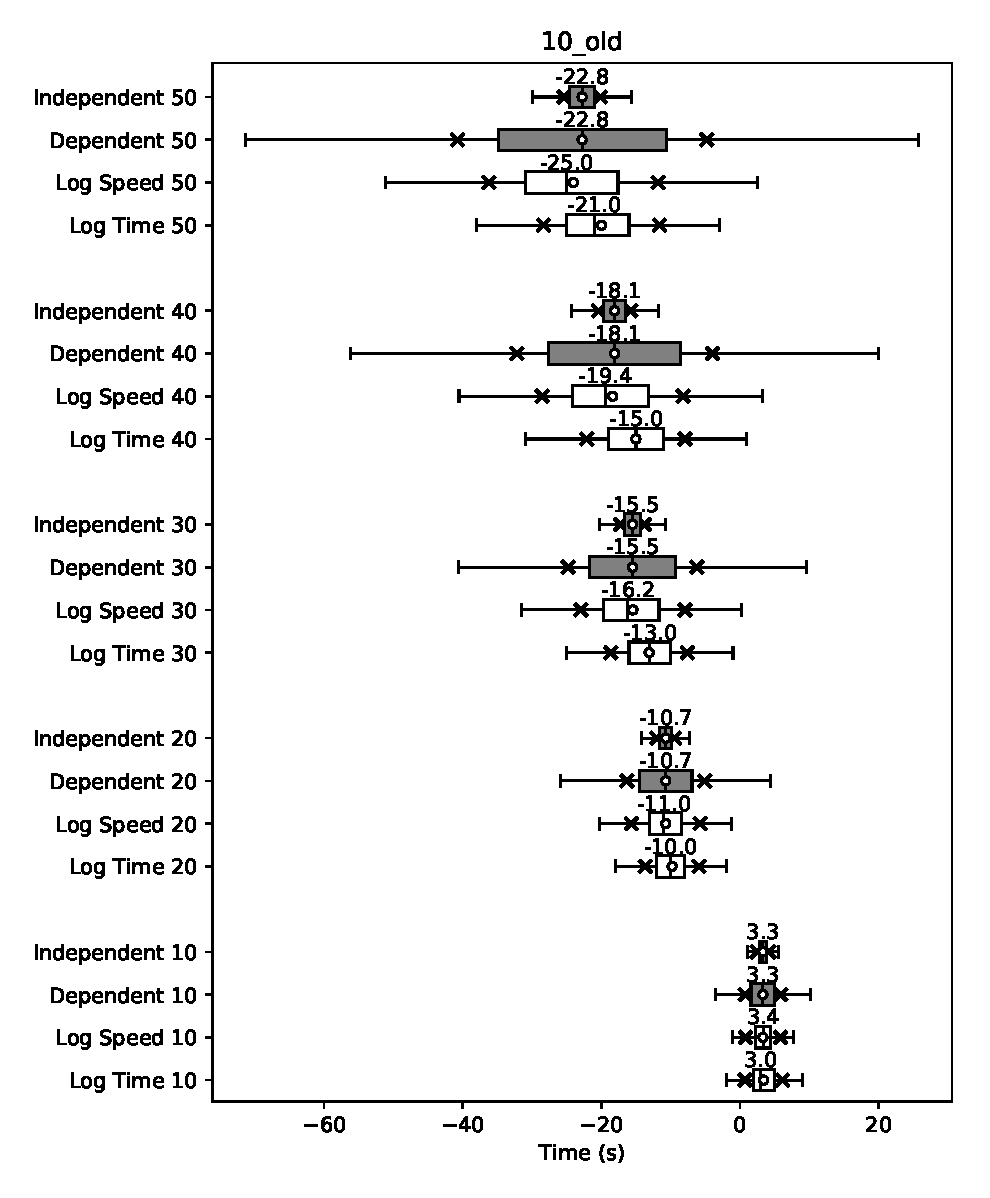
\includegraphics[height=0.8\textheight]{10_old.eps}
	\end{frame}
	\begin{frame}
		\frametitle{Appendix - Low Data Time Differences}
		\hspace{1.6cm}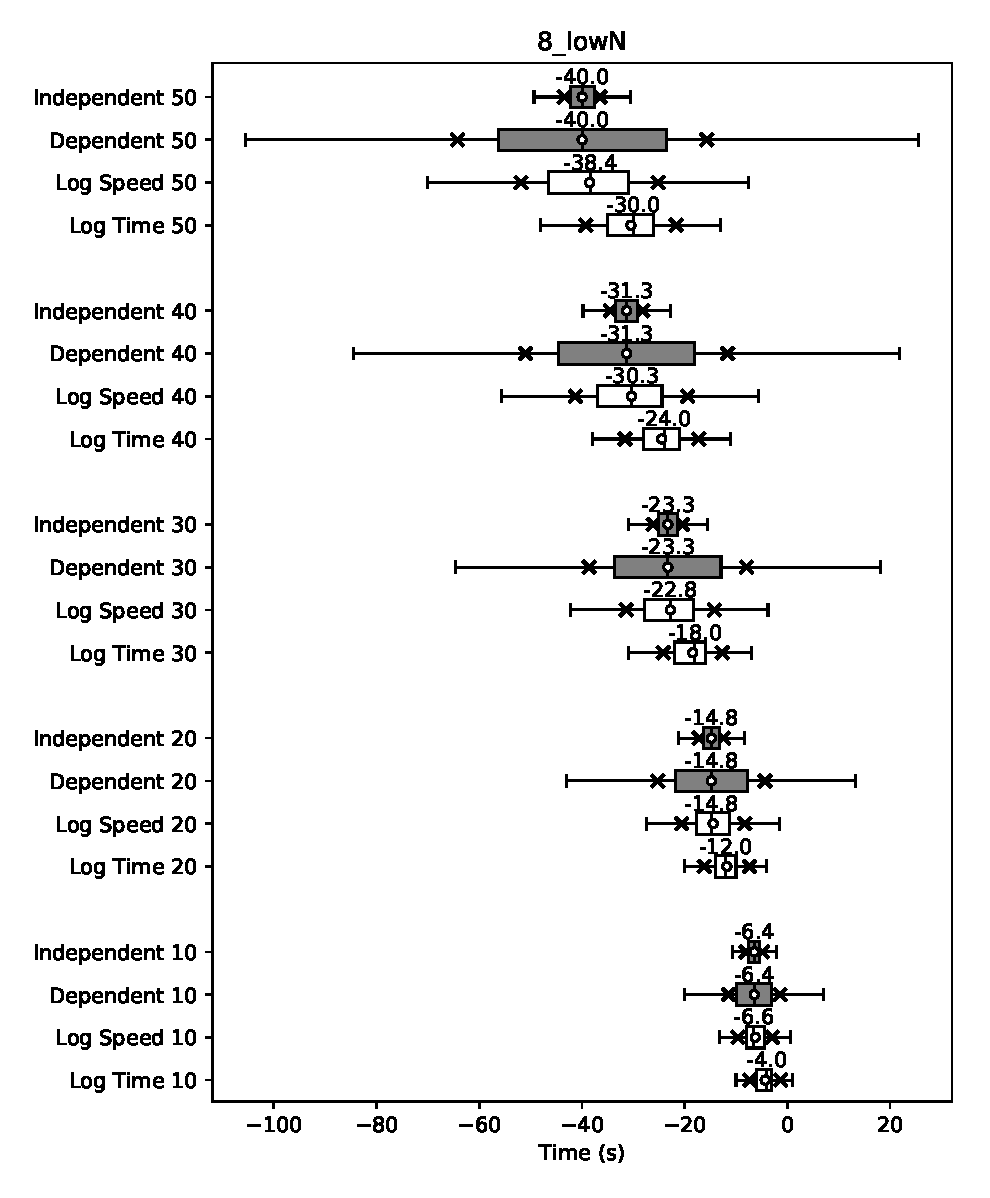
\includegraphics[height=0.8\textheight]{8_lowN.eps}
	\end{frame}


\end{document}
